\documentclass[conference]{IEEEtran}
\IEEEoverridecommandlockouts

\usepackage{cite}
\usepackage{amsmath,amssymb,amsfonts}
\usepackage{graphicx}
\usepackage{textcomp}
\usepackage{xcolor}
\usepackage{booktabs}
\usepackage{url}
\usepackage{pgfplots}
\pgfplotsset{compat=1.18}
\usetikzlibrary{arrows.meta,positioning,fit}

\newcommand{\cbha}{\textsc{cbha}}
\newcommand{\kbps}{\,kbit/s}

\begin{document}

\title{Department-Aware Arbitration of Contended Enterprise Network Slices on a Live Traffic Testbed}

\author{
\IEEEauthorblockN{Thrishwant G}
\IEEEauthorblockA{\textit{[Department]} \\
\textit{[Institution]}\\
City, Country \\
email@institution.edu}
\and
\IEEEauthorblockN{K Jaya Sai Venkatesh}
\IEEEauthorblockA{\textit{[Department]} \\
\textit{[Institution]}\\
City, Country \\
email@institution.edu}
\and
\IEEEauthorblockN{Hithesh Y}
\IEEEauthorblockA{\textit{[Department]} \\
\textit{[Institution]}\\
City, Country \\
email@institution.edu}
\and
\IEEEauthorblockN{K J Sathya Prathmesh}
\IEEEauthorblockA{\textit{[Department]} \\
\textit{[Institution]}\\
City, Country \\
email@institution.edu}
}

\maketitle

\begin{abstract}
Enterprise networks provision more slice bandwidth than their links can carry. When demand peaks together, a shared bottleneck queue fills and every slice suffers, including the ones the business can least afford to lose; a generic controller then degrades slices by provisioning-time labels such as slice type or a static priority. We built a small but real testbed to study runtime arbitration under these conditions. Phones and laptops join one of seven department slices over a laptop's Wi-Fi hotspot; every byte they download passes through an application-layer gateway that enforces a per-slice token bucket in front of a shared 1\,Mbit/s link and measures throughput, drops and probe round-trip latency every 2\,s. A controller reads these measurements, detects contention, chooses new limits with Convex Business-Harm Arbitration (\cbha{}), a marginal-harm water-filling method driven by department business attributes and hard compliance ceilings, and pushes them back to the gateway, recording an auditable explanation for every decision. On a loopback run of six automated test cases, all checks pass. Under a lunch-hour overload of 1{,}316\kbps{} on a 950\kbps{} link, switching arbitration on cut the 95th-percentile latency of the clinic, factory and laboratory slices from about 505\,ms to 22--23\,ms and their loss from up to 21\% to zero, while a signage slice labelled URLLC was held at its 28\kbps{} floor. We also show that weighted fair queueing without a controller protects light slices but is business-blind: at full peak it gives the life-safety clinic 37.5\kbps{}, below its 40\kbps{} contractual floor.
\end{abstract}

\begin{IEEEkeywords}
network slicing, enterprise networks, testbed, token bucket, deficit round robin, resource arbitration, SLA, explainability
\end{IEEEkeywords}

\section{Introduction}

Network slicing divides one physical network into logical networks, each with its own service-level agreement (SLA) on throughput, latency and loss~\cite{ngmn2015,foukas2017,afolabi2018}. Enterprise and private 5G sites use it to separate clinical telemetry, production control, laboratory instruments, video surveillance, office traffic and building services on one site network. Slices are given a guaranteed floor and a nominal (baseline) share, and the baselines deliberately add up to more than the link: statistical multiplexing makes this efficient because departments rarely peak together. When they do, the network is \emph{contended}.

Two things then go wrong. First, without any arbitration the shared bottleneck queue fills and \emph{every} slice waits behind it, so even a slice that sends far less than its share sees its latency rise to the length of the buffer~\cite{gettys2012}. Second, when a controller does intervene, it usually ranks slices by network attributes fixed at provisioning time: the slice/service type, the 5QI of its flows or a static priority integer~\cite{3gpp23501,3gpp23503}. These labels describe traffic behaviour, not what the enterprise depends on. In the enterprise we use throughout this paper, canteen digital signage was provisioned as URLLC, the same type as patient telemetry, while a regulated quality laboratory was provisioned as eMBB; a label-based controller protects the signage and cuts the laboratory.

Our companion work formulated arbitration as minimisation of a convex \emph{business-harm} function under hard compliance constraints and evaluated it in simulation. Simulation leaves open whether the method works on real traffic: whether measured demand and latency are good enough inputs, whether the control loop is fast and stable, and whether cutting the right slices actually restores the protected ones. This paper answers those questions on a live testbed. Our contributions are:
\begin{itemize}
\item A low-cost slicing testbed in which real devices on a Wi-Fi hotspot generate traffic through an application-layer gateway with per-slice token buckets, a shared bottleneck and in-band latency probes, controlled through a small southbound API (Section~\ref{sec:testbed}).
\item The integration of \cbha{} into a closed loop on measured data, including a shortage estimate based on carried rather than requested traffic (Section~\ref{sec:model}).
\item Six reproducible test cases and an A/B experiment that quantifies what arbitration buys on the wire, with every 2\,s measurement window recorded (Sections~\ref{sec:setup}--\ref{sec:results}).
\item A comparison with weighted fair queueing (deficit round robin) without a controller, showing where it is sufficient and where it breaks a business rule (Section~\ref{sec:drr}).
\end{itemize}

\section{Background and Related Work}

\textit{Slicing and QoS.} Surveys by Foukas \textit{et al.}~\cite{foukas2017} and Afolabi \textit{et al.}~\cite{afolabi2018} cover slicing architectures and isolation. 3GPP defines slice identity in TS~23.501~\cite{3gpp23501} and per-session aggregate maximum bit rates in TS~23.503~\cite{3gpp23503}; the GSMA template describes slices by network attributes~\cite{gsma_gst}. Differentiated Services~\cite{rfc2475} classifies traffic into a small number of behaviour classes. None of these carries the business context of the department that owns a slice.

\textit{Shaping and scheduling.} Per-flow rate limits are enforced with token (leaky) buckets~\cite{turner1986}. Fair queueing~\cite{demers1989} and its efficient approximation, deficit round robin (DRR)~\cite{shreedhar1996}, share a bottleneck among queues in proportion to weights and isolate a light flow from heavy ones. Large FIFO buffers at a bottleneck cause persistent queueing delay (bufferbloat)~\cite{gettys2012}, which active queue management such as CoDel addresses~\cite{nichols2012}. These mechanisms decide how a link is shared \emph{given} the limits; they do not decide which department should give up bandwidth.

\textit{Allocation and testbeds.} Multi-tenant slice allocation has been studied as a game among tenants~\cite{caballero2019} and as forecasting-driven admission~\cite{sciancalepore2017}; separable convex resource allocation is solved by greedy marginal allocation~\cite{ibaraki1988} and water-filling~\cite{palomar2005}. Emulated testbeds such as Mininet~\cite{lantz2010} and open 5G stacks~\cite{open5gs,ueransim} run real protocol code but need Linux hosts and radio emulation. Our testbed trades realism of the radio for the ability to use unmodified phones and a single Windows laptop.

\section{Arbitration Model}
\label{sec:model}

We summarise \cbha{} as used here; the companion work gives the derivation. There are $n$ slices on an offered capacity $C$. Slice $i$ has baseline $b_i$, floor $f_i$, current limit $a_i$ and measured demand $D_i$, and belongs to a department with seven business attributes: criticality, downtime cost per minute $c_i$, business importance, compliance level, customer impact, operational importance and recovery tolerance.

\textit{Business priority score.} Each attribute is mapped to $[0,100]$ and combined with policy weights (0.26, 0.20, 0.16, 0.14, 0.12, 0.07, 0.05 in the order above) into a score $B_i$; downtime cost is normalised logarithmically so no single department can saturate the score by claiming an extreme cost. Compliance also sets a hard ceiling $M_i$ on how deep a slice may be cut: 0\% for life-safety, at most 20\% for regulated, otherwise the department's declared limit.

\textit{Harm and problem.} Cutting slice $i$ by a fraction $d_i$ of its baseline causes harm
\begin{equation}
H_i(d_i) = B_i \left(d_i / M_i\right)^{\gamma_i} S_i\, F_i\, U_i\, I_i ,
\label{eq:harm}
\end{equation}
where the curvature $\gamma_i \in \{3.0, 2.2, 1.6, 1.15\}$ follows recovery tolerance (zero to high), $S_i$ rises with live SLA stress, $F_i$ is a bounded fairness term for slices that were cut recently, $U_i$ converts expected hold time and downtime cost into urgency and $I_i$ scales by recovery intolerance. \cbha{} solves
\begin{equation}
\min_{\mathbf d} \textstyle\sum_i H_i(d_i) \;\; \text{s.t.} \;\; \sum_i r_i(d_i) \ge \Delta, \;\; 0 \le d_i \le \bar d_i ,
\label{eq:p1}
\end{equation}
with $\bar d_i = \min(M_i, (a_i - f_i)/b_i)$, by releasing bandwidth in small quanta to whichever slice has the lowest marginal harm per kbit/s freed. For $\gamma_i \ge 1$ the problem is convex and this greedy water-filling is optimal up to the quantum~\cite{ibaraki1988,boyd2004}. Life-safety slices ($M_i = 0$) are removed before optimisation, so no weighting can reach them.

\textit{Shortage on measured traffic.} On a real link a slice can never carry more than its limit, and the excess it requests is dropped at its own queue. Cutting the limit of a slice that already sends less than its new limit frees nothing. We therefore compute the shortage from carried traffic,
\begin{equation}
\Delta = \textstyle\sum_i \min(D_i, a_i) - (1-h)\,C ,
\end{equation}
with headroom $h = 3\%$, and count as freed $r_i$ only the part of a cut below $\min(D_i, a_i)$. A cut of a slice that cannot help is never chosen. When the ceilings do not allow $\Delta$ to be freed, \cbha{} frees what policy permits, reports a \textsc{partial} verdict with the shortfall and alerts the operator instead of breaking a rule.

\textit{Explanation.} Every decision prices four alternative strategies on the same harm function (priority sort, uniform cut, single victim, protect-stressed), stores per-slice reasons that name concrete values, a confidence score, and the resolved policy version, and is written to an append-only audit log.

\section{Testbed Design}
\label{sec:testbed}

Fig.~\ref{fig:arch} shows the testbed. All components are TypeScript on Node.js and run on one Windows laptop; devices need only a web browser.

\begin{figure}[t]
\centering
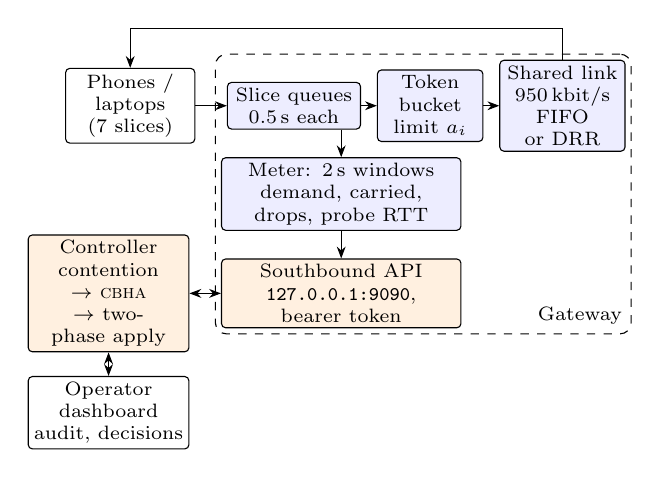
\begin{tikzpicture}[
  node distance=2.6mm,
  box/.style={draw, rounded corners=1.5pt, align=center, font=\scriptsize, minimum height=5mm, fill=white, inner sep=2pt},
  data/.style={box, fill=blue!7},
  ctl/.style={box, fill=orange!12},
  >={Stealth[length=1.5mm]}
]
\node[box, text width=1.5cm] (dev) {Phones / laptops\\(7 slices)};
\node[data, right=4mm of dev, text width=1.55cm] (sq) {Slice queues\\0.5\,s each};
\node[data, right=2mm of sq, text width=1.2cm] (tb) {Token bucket\\limit $a_i$};
\node[data, right=2mm of tb, text width=1.45cm] (root) {Shared link\\950\kbps{}\\FIFO or DRR};
\node[data, below=3.5mm of sq, text width=2.9cm, xshift=6mm] (meter) {Meter: 2\,s windows\\demand, carried, drops, probe RTT};
\node[ctl, below=3.5mm of meter, text width=2.9cm] (api) {Southbound API\\\texttt{127.0.0.1:9090}, bearer token};
\node[ctl, left=4mm of api, text width=1.9cm] (ctrl) {Controller\\contention $\rightarrow$ \cbha{}\\$\rightarrow$ two-phase apply};
\node[box, below=3mm of ctrl, text width=1.9cm] (dash) {Operator dashboard\\audit, decisions};
\draw[->] (dev) -- (sq);
\draw[->] (sq) -- (tb);
\draw[->] (tb) -- (root);
\draw[->] (root.north) -- ++(0,4mm) -| (dev.north);
\draw[->] (sq.south) ++(6mm,0) -- (meter.north);
\draw[->] (meter) -- (api);
\draw[<->] (api) -- (ctrl);
\draw[<->] (ctrl) -- (dash);
\node[draw, dashed, rounded corners, fit=(sq)(tb)(root)(meter)(api), inner sep=2pt, label={[font=\scriptsize, anchor=south east]south east:Gateway\ }] {};
\end{tikzpicture}
\caption{The testbed. Devices reach the gateway over HTTP on port 8080; every byte they download passes through the slice queue, its token bucket and the shared link, and returns with the probe replies (top arrow). The controller only reads measurement windows and writes limits through the southbound API.}
\label{fig:arch}
\end{figure}

\subsection{Gateway data path}
A device joins a slice with a six-character join code (or a QR code shown on the dashboard) and opens a streaming download whose rate it chooses: that rate is the slice's \emph{demand}. Every 20\,ms the gateway's scheduler runs three steps. \emph{Arrivals}: each session puts the bytes it requested into its slice queue in chunks of at most 1\,KB; a full queue tail-drops. \emph{Policing}: a per-slice token bucket releases bytes at no more than the slice's limit; its depth is $\max(0.1\,\text{s}\cdot a_i, 1\,\text{KB})$, so that a slice cut to a few kbit/s can still send a full chunk. \emph{Transmit}: a root token bucket drains the link at the offered capacity. With the default \textsc{fifo} discipline, policed chunks wait in one shared queue holding 0.5\,s of link traffic, as in a plain switch port. With \textsc{drr}, each slice's queue is served directly by weighted deficit round robin~\cite{shreedhar1996}, with a quantum of 20\,ms of traffic at the slice's limit. Each slice queue holds 0.5\,s of traffic at the slice's \emph{current} limit and is resized whenever the limit changes. Rates are computed from real elapsed time, so Windows timer jitter does not change them.

\subsection{Measurement}
Each device sends a small probe through the same slice queue as its data (every second from a phone, every 0.5\,s from the test agents), so the probe's round-trip time is the latency the slice's traffic actually sees. The gateway closes a measurement window every 2\,s on a timer and keeps, per slice: demand, carried and dropped rate, queueing delay, probe latency p50 and p95, jitter, loss and availability. Loss is the larger of the dropped share of offered bytes and the share of unanswered probes; an unknown value is reported as unknown, never as zero. \texttt{GET /v1/stats} returns the last completed window and is read-only, so the controller, the dashboard and the recorder all see the same numbers.

\subsection{Control loop}
The controller polls the gateway every 2\,s. A contention opens after two consecutive windows in which demand exceeds 102\% of offered capacity, and closes after three windows below it; a 20\,s cooldown separates decisions. On a decision, slice updates, the decision record and its audit entry commit together, and the new limits are then pushed with \texttt{PUT /v1/slices/:code/limit}; a refusal is reconciled to the value the gateway reports. Degraded slices return to baseline when their department's recovery window (30\,s to 30\,min) expires or when an administrator overrides the decision with a stated reason. If the gateway restarts, the controller detects the lower uptime and re-sends the slice catalogue with the current limits.

\subsection{Devices, operator and scale}
Devices connect to the laptop's Windows Mobile Hotspot (at most eight clients) and open the department page served by the gateway on port 8080; the southbound port is bound to loopback. The page shows the slice's limit, demand, carried rate, latency and, when the slice is cut, the controller's explanation. An operator can set a slice's demand remotely, run a scenario that sets all slices at once, turn automatic arbitration off and on, remove a device and download the recording. The link is scaled to 1\,Mbit/s so that seven phones on one hotspot can overload it without the Wi-Fi itself becoming the bottleneck; the engine's bandwidth unit is mapped to 1\kbps.

\section{Experimental Setup}
\label{sec:setup}

\begin{table}[t]
\caption{The enterprise: seven slices on a 950\kbps{} link}
\label{tab:slices}
\centering
\footnotesize
\setlength{\tabcolsep}{3pt}
\begin{tabular}{@{}llrrrrr@{}}
\toprule
Slice (department) & Label & $b_i$ & $f_i$ & $M_i$ & $B_i$ & SLA p95 \\
\midrule
Patient telemetry (Clinic) & URLLC & 60 & 40 & 0\% & 96.0 & 150\,ms \\
Factory automation & URLLC & 380 & 170 & 15\% & 81.7 & 180\,ms \\
Lab instrumentation & eMBB & 180 & 50 & 20\% & 70.9 & 500\,ms \\
Warehouse operations & URLLC & 160 & 55 & 35\% & 59.1 & 250\,ms \\
CCTV (Security) & eMBB & 240 & 60 & 40\% & 48.8 & 900\,ms \\
Office Wi-Fi (Office IT) & eMBB & 320 & 70 & 45\% & 43.4 & 600\,ms \\
Canteen signage & URLLC & 140 & 28 & 80\% & 8.0 & 350\,ms \\
\midrule
Total & & 1480 & 473 & & & \\
\bottomrule
\end{tabular}
\\[2pt]\raggedright\scriptsize Rates in kbit/s. $M_i$: maximum cut. $B_i$: business priority score.
\end{table}

Table~\ref{tab:slices} lists the slices. Baselines total 1{,}480\kbps{}, 1.56 times the 950\kbps{} offered by the 1\,Mbit/s link (50\kbps{} reserved); floors total 473\kbps{}, so the floors alone always fit. Note the label inversions: Canteen and Warehouse are URLLC but have low business scores, and the regulated Lab is eMBB.

\begin{table}[t]
\caption{Test cases (demand as a fraction of baseline)}
\label{tab:tcs}
\centering
\footnotesize
\setlength{\tabcolsep}{3pt}
\begin{tabular}{@{}p{1.75cm}p{3.0cm}p{3.0cm}@{}}
\toprule
Case & Load & Pass criteria \\
\midrule
TC1 Normal day & all 55\% (814\kbps{}) & no contention, no cut, loss $<$1\% \\
TC2 Canteen flood & Canteen 200\%, rest 55\% & Canteen held at its limit; no limit changes \\
TC3 Lunch rush & Canteen 200\%, Office, CCTV 100\%, Warehouse 80\%, rest 55\% (1{,}316\kbps{}) & decision enforced; Clinic not cut; floors and ceilings kept; protected slices within SLA \\
TC4 Peak & all 100\% (1{,}480\kbps{}) & \textsc{partial} verdict and alert; Clinic not cut \\
TC5 Recovery & back to 55\% & contention closes; recovery scheduled; override restores baselines \\
TC6 A/B & TC3 load, arbitration off then on & lower p95, no higher loss for Clinic, Factory, Lab \\
\bottomrule
\end{tabular}
\end{table}

Table~\ref{tab:tcs} lists the test cases. An automated driver (\texttt{npm run demo:local}) starts the gateway and controller on one laptop, joins one software agent per slice over loopback, runs TC1--TC6 and checks every criterion from the recorded windows. In TC6 each phase has a 25\,s warm-up followed by 40\,s (20 windows) of measurement. Unless stated, the link uses \textsc{fifo}. The agents use the same join, load and probe API as the phones; the hotspot run with phones is described in the repository's runbook and is not part of the measurements below.

\section{Results}
\label{sec:results}

\subsection{Shaper accuracy}
We drove a single saturated slice (demand twice its limit) for 10\,s of virtual time with uneven ticks of 20, 35 and 50\,ms, imitating Windows timers. The carried rate was within 0.25\% of the limit at every tested limit (Table~\ref{tab:shaper}), including the 28\kbps{} floor of the canteen slice.

\begin{table}[t]
\caption{Shaper accuracy on a saturated slice}
\label{tab:shaper}
\centering
\footnotesize
\begin{tabular}{@{}lrrrrrr@{}}
\toprule
Limit (kbit/s) & 20 & 28 & 60 & 140 & 380 & 950 \\
Error (\%) & 0.00 & $-$0.21 & 0.10 & 0.25 & $-$0.03 & 0.03 \\
\bottomrule
\end{tabular}
\end{table}

\subsection{Test cases TC1--TC5}
All checks passed. In TC1 every slice carried its demand with p95 latency of 22--37\,ms and no loss. In TC2 the canteen asked for 278\kbps{} and its own token bucket held it at 139\kbps{}; the canteen alone saw queueing (p95 465\,ms, 50\% loss), the other six slices kept p95 below 30\,ms, and the engine made no change because the carried total (877\kbps{}) still fitted the link: the per-slice limit already isolates a single flooding department.

In TC3 demand rose to 1{,}316\kbps{}, and the carried total that the limits allow to 1{,}173\kbps{}, a shortage of 251.5\kbps{} against the 921.5\kbps{} target. A contention was already open from TC2 (demand above 102\% of capacity, but nothing worth freeing), and new limits were enforced 4.0\,s after the TC3 load started. \cbha{} cut Canteen to its 28\kbps{} floor ($-$80\%), Office to 217\kbps{}, CCTV to 211\kbps{} and Warehouse to 121\kbps{}, and left Clinic, Factory and Lab untouched. The cut slices carried exactly their new limits; Clinic, Factory and Lab ran at 21--29\,ms p95 with no loss. The URLLC label of the canteen did not protect it, and the eMBB label of the lab did not expose it.

In TC4 every slice demanded its full baseline. The ceilings allow at most 501\kbps{} to be freed against a 558.5\kbps{} shortage, so the engine reported \textsc{partial}, cut every slice except the clinic to its ceiling and alerted the operator. Because the link stays overloaded by about 30\kbps{}, every slice queued (p95 0.6--1.1\,s), the honest outcome when policy forbids a feasible plan. The clinic, which demanded slightly more than its own 60\kbps{} limit, was held at that limit and was never cut. In TC5 the contention closed after three windows below the threshold, a recovery time was scheduled for every degraded slice, and an administrator override restored all baselines.

\subsection{Arbitration off versus on (TC6)}

\begin{table}[t]
\caption{TC6: lunch-rush load, arbitration off vs.\ on (FIFO link, means of 20 windows)}
\label{tab:tc6}
\centering
\footnotesize
\setlength{\tabcolsep}{3pt}
\begin{tabular}{@{}lrrrrr@{}}
\toprule
 & \multicolumn{2}{c}{p95 latency (ms)} & \multicolumn{2}{c}{Loss (\%)} & Limit on \\
Slice & off & on & off & on & (kbit/s) \\
\midrule
Clinic & 503 & \textbf{23} & 5.62 & \textbf{0} & 60 \\
Factory & 509 & \textbf{22} & 21.47 & \textbf{0} & 380 \\
Lab & 505 & \textbf{22} & 14.99 & \textbf{0} & 180 \\
Warehouse & 507 & 475 & 18.29 & 5.23 & 122 \\
CCTV & 626 & 479 & 17.53 & 14.88 & 204 \\
Office & 573 & 476 & 19.81 & 31.19 & 221 \\
Canteen & 949 & 415 & 65.15 & 90.03 & 28 \\
\bottomrule
\end{tabular}
\end{table}

\begin{figure}[t]
\centering
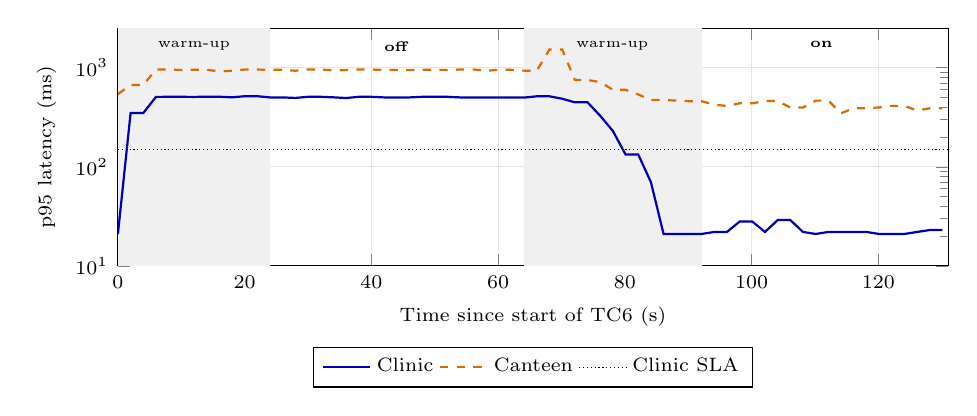
\begin{tikzpicture}
\begin{axis}[
  width=\columnwidth, height=4.6cm,
  ymode=log, ymin=10, ymax=2500,
  xmin=0, xmax=131,
  xlabel={Time since start of TC6 (s)}, ylabel={p95 latency (ms)},
  label style={font=\scriptsize}, tick label style={font=\scriptsize},
  legend style={font=\scriptsize, at={(0.5,-0.34)}, anchor=north, legend columns=3},
  grid=major, grid style={gray!20},
]
\fill[gray!12] (axis cs:0,10) rectangle (axis cs:24,2500);
\fill[gray!12] (axis cs:64.1,10) rectangle (axis cs:92.1,2500);
\node[font=\tiny, anchor=north] at (axis cs:12,2300) {warm-up};
\node[font=\tiny, anchor=north] at (axis cs:44,2300) {\textbf{off}};
\node[font=\tiny, anchor=north] at (axis cs:78,2300) {warm-up};
\node[font=\tiny, anchor=north] at (axis cs:111,2300) {\textbf{on}};
\addplot[thick, blue!70!black, mark=none] coordinates {(0,21) (2,348) (4,348) (6,507) (8,508) (10,508) (12,507) (14,509) (16,509) (18,502) (20,515) (22,515) (24,501) (26,501) (28,495) (30,508) (32,508) (34,502) (36,494) (38,508) (40,508) (42,501) (44,501) (46,501) (48,508) (50,508) (52,508) (54,501) (56.1,501) (58.1,501) (60.1,499) (62.1,499) (64.1,499) (66.1,514) (68.1,514) (70.1,486) (72.1,447) (74.1,447) (76.1,327) (78.1,230) (80.1,133) (82.1,133) (84.1,70) (86.1,21) (88.1,21) (90.1,21) (92.1,21) (94.1,22) (96.1,22) (98.1,28) (100.1,28) (102.1,22) (104.1,29) (106.1,29) (108.1,22) (110.1,21) (112.1,22) (114.1,22) (116.1,22) (118.1,22) (120.1,21) (122.1,21) (124.1,21) (126.1,22) (128.1,23) (130.1,23)};
\addlegendentry{Clinic}
\addplot[thick, orange!85!black, dashed, mark=none] coordinates {(0,542) (2,667) (4,667) (6,959) (8,959) (10,945) (12,952) (14,952) (16,916) (18,930) (20,957) (22,957) (24,951) (26,951) (28,931) (30,958) (32,958) (34,938) (36,945) (38,959) (40,959) (42,945) (44,945) (46,944) (48,952) (50,952) (52,944) (54,959) (56.1,959) (58.1,930) (60.1,951) (62.1,951) (64.1,933) (66.1,932) (68.1,1528) (70.1,1528) (72.1,751) (74.1,751) (76.1,715) (78.1,598) (80.1,598) (82.1,536) (84.1,472) (86.1,472) (88.1,465) (90.1,459) (92.1,459) (94.1,423) (96.1,411) (98.1,437) (100.1,437) (102.1,460) (104.1,460) (106.1,397) (108.1,396) (110.1,465) (112.1,465) (114.1,347) (116.1,390) (118.1,390) (120.1,397) (122.1,411) (124.1,411) (126.1,370) (128.1,389) (130.1,389)};
\addlegendentry{Canteen}
\addplot[thin, black, densely dotted, domain=0:131] {150};
\addlegendentry{Clinic SLA}
\end{axis}
\end{tikzpicture}
\caption{TC6 time series. With arbitration off the shared queue is full and the clinic waits about 0.5\,s. After arbitration is switched on (64\,s) the cheap slices are cut and the shared queue drains in about 20\,s.}
\label{fig:tc6ts}
\end{figure}

Table~\ref{tab:tc6} and Fig.~\ref{fig:tc6ts} show the A/B experiment. With arbitration off, the carried total sits at the link rate (940--960\kbps{}) and the shared FIFO stays full. Every slice waits about one buffer length, 0.5\,s, regardless of how little it sends; the clinic, which uses only 34 of its 60\kbps{}, loses 5.6\% of its traffic and is more than three times over its 150\,ms target. With arbitration on, the engine makes the same kind of decision as in TC3, carried traffic falls to about 920\kbps{} (the 3\% headroom), and Clinic, Factory and Lab return to 22--23\,ms p95 with zero loss, a 22-fold reduction. The tail-drop loss is moved onto the slices the business chose to cut: Office and Canteen lose more than before, because their limits are now below their demand.

The slices that were cut still show about 475\,ms p95. That is not shared-queue delay: each now waits in its \emph{own} slice queue, which holds 0.5\,s at its new limit and is permanently full because its demand exceeds its limit. The canteen's latency is lower than with arbitration off because it no longer waits behind the shared queue as well.

\textit{Recovery time.} The protected slices took about 22\,s to recover after arbitration was switched on (Fig.~\ref{fig:tc6ts}): roughly 4\,s to detect and decide and 18\,s to drain. The drain time follows from the design: the shared buffer holds $0.5\,\text{s} \times 950 = 475$\,kbit and, after the cut, drains at only the headroom, $950 - 921 \approx 29$\kbps{}, so it needs about 16\,s. A larger headroom or a smaller buffer would shorten recovery at the cost of utilisation; active queue management~\cite{nichols2012} at the shared link would remove most of the standing queue.

\begin{figure}[t]
\centering
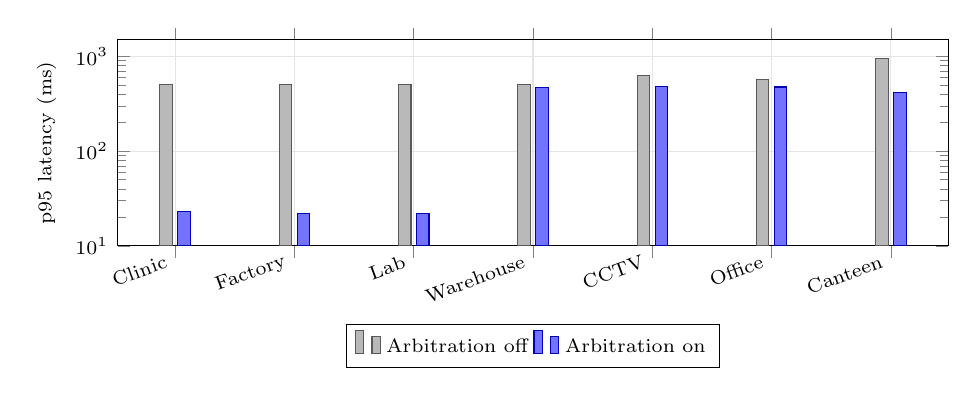
\begin{tikzpicture}
\begin{axis}[
  ybar, bar width=4.5pt,
  width=\columnwidth, height=4.2cm,
  ymode=log, ymin=10, ymax=1500, log origin=infty,
  symbolic x coords={Clinic,Factory,Lab,Warehouse,CCTV,Office,Canteen},
  xtick=data, x tick label style={font=\scriptsize, rotate=20, anchor=east},
  ylabel={p95 latency (ms)}, label style={font=\scriptsize}, tick label style={font=\scriptsize},
  legend style={font=\scriptsize, at={(0.5,-0.38)}, anchor=north, legend columns=2},
  grid=major, grid style={gray!20}, enlarge x limits=0.08,
]
\addplot[fill=gray!55, draw=gray!70!black] coordinates {(Clinic,503) (Factory,509) (Lab,505) (Warehouse,507) (CCTV,626) (Office,573) (Canteen,949)};
\addplot[fill=blue!55, draw=blue!70!black] coordinates {(Clinic,23) (Factory,22) (Lab,22) (Warehouse,475) (CCTV,479) (Office,476) (Canteen,415)};
\legend{Arbitration off, Arbitration on}
\end{axis}
\end{tikzpicture}
\caption{p95 latency per slice under the lunch-rush load (means of 20 windows).}
\label{fig:tc6bars}
\end{figure}

\subsection{Is fair queueing enough?}
\label{sec:drr}

The FIFO result raises an obvious question: would weighted fair queueing at the link, with no controller at all, give the same protection? We ran the real gateway scheduler on a virtual clock with every slice at its baseline limit, for the TC3 and TC4 loads (Table~\ref{tab:drr}).

\begin{table}[t]
\caption{No controller: carried rate (kbit/s) and probe p95 (ms) with every slice at its baseline limit}
\label{tab:drr}
\centering
\footnotesize
\setlength{\tabcolsep}{2.6pt}
\begin{tabular}{@{}lrrrr|rrrr@{}}
\toprule
 & \multicolumn{4}{c|}{TC3 lunch rush} & \multicolumn{4}{c}{TC4 everyone at peak} \\
 & \multicolumn{2}{c}{FIFO} & \multicolumn{2}{c|}{DRR} & \multicolumn{2}{c}{FIFO} & \multicolumn{2}{c}{DRR} \\
Slice & kb/s & ms & kb/s & ms & kb/s & ms & kb/s & ms \\
\midrule
Clinic & 31.6 & 500 & 33.2 & 40 & 51.8 & 960 & \textbf{37.5} & 760 \\
Factory & 163.8 & 500 & 209.3 & 40 & 215.3 & 560 & 243.0 & 760 \\
Lab & 86.9 & 500 & 99.2 & 40 & 132.6 & 740 & 114.6 & 760 \\
Warehouse & 102.8 & 500 & 111.7 & 700 & 119.0 & 780 & 101.7 & 760 \\
CCTV & 207.6 & 660 & 167.9 & 700 & 137.6 & 660 & 153.0 & 760 \\
Office & 253.1 & 600 & 224.2 & 680 & 182.1 & 600 & 204.3 & 760 \\
Canteen & 97.6 & 960 & 97.6 & 700 & 105.8 & 820 & 88.8 & 760 \\
\bottomrule
\end{tabular}
\end{table}

Under the lunch rush, DRR alone protects Clinic, Factory and Lab: each sends less than its weighted share, so it never waits behind another slice's backlog (p95 40\,ms, i.e.\ two scheduler ticks on the virtual clock). This is the isolation fair queueing is designed for~\cite{demers1989,shreedhar1996}, and it is a strong argument for using it under any controller. But DRR shares by weight, not by business value. The canteen keeps 97.6\kbps{}, three and a half times its floor, while the warehouse, with a much higher business score, is squeezed below its demand. At full peak (TC4), DRR gives every slice its proportional share, $950 \cdot b_i / 1480$: the life-safety clinic receives 37.5\kbps{}, below its 40\kbps{} contractual floor and in breach of its 0\% ceiling, and every queue in the gateway is full. No choice of weights fixes this in general, because the right answer depends on which departments are active.

We repeated all six test cases on the testbed with the DRR link (\texttt{paper/results/drr-demo-local.csv}). TC1--TC5 passed. TC6 failed one check by design: with DRR the protected slices were already at 32--40\,ms p95 with arbitration off, so switching it on could not lower their latency further. What arbitration changed was \emph{who pays}: the canteen fell from 99 to its 28\kbps{} floor and the warehouse, CCTV and office loss dropped (13.0$\rightarrow$5.3\%, 30.0$\rightarrow$16.5\%), with the same engine decision as on FIFO. Fair queueing and business-aware arbitration are therefore complementary: DRR isolates slices within their share, \cbha{} decides the shares.


\section{Discussion and Limitations}
\label{sec:disc}

\textit{Loopback, not Wi-Fi.} The measurements above use software agents on the same laptop as the gateway. They exercise the real gateway, measurement and control loop, but not the wireless hop. The 21--22\,ms floor of the latency results is almost entirely the gateway's 20\,ms scheduler tick. The phone run on the hotspot is supported (QR join, per-tab identity, automatic rejoin after a gateway restart, firewall scripts, a session recorder) but its results are future work; on Wi-Fi we expect a higher and noisier latency floor and the same queueing behaviour at the gateway.

\textit{Application-layer slicing.} The gateway shapes traffic it generates itself, at the application layer, in Node.js. It is not kernel traffic control, not 3GPP radio slicing, and its token buckets are not per-packet policers. An optional forward proxy admits joined devices' own traffic but does not shape it yet, and only downlink load is generated. The scaled 1\,Mbit/s link keeps the Wi-Fi from being the bottleneck; results at higher rates would need a native shaper.

\textit{Demand is observable here.} The gateway sees the rate each device requests before policing, which a real network does not: once a slice is capped it reports throughput at the cap. Our carried-traffic shortage partly addresses this, but a deployment would have to estimate demand from drops and queue signals.

\textit{Harm model.} \cbha{} is optimal for its own harm function. The testbed shows that its decisions have the intended effect on the wire; it does not show that the harm function matches what each department would actually lose, which needs calibration against real outages.

\section{Conclusion}

A small testbed with real traffic, a shaped shared link and in-band probes is enough to show both halves of the contended-slice problem. Without arbitration, a full shared queue gives every department half a second of delay and real loss, the clinic included. With department-aware arbitration, the controller detects the overload within seconds, cuts the slices the business values least within their policy ceilings, restores the protected slices to their unloaded latency with zero loss, and records why. Fair queueing is a valuable complement, since it isolates slices that stay within their share, but it cannot decide who should give way at peak and can break a contractual floor. Next steps are the hotspot run with seven phones, a native kernel shaper at higher rates, active queue management at the shared link and demand estimation from capped traffic.

\section*{Code and Data Availability}
The testbed, the test driver, the raw 2\,s measurement windows behind every table and figure, and the scripts that produce them are available at [repository URL].

\bibliographystyle{IEEEtran}
\bibliography{references}

\end{document}
